\chapter{Color-Ordered Feynman Rules}
\label{sec:cofr}

For completeness, we provide the QCD color-ordered Feynman rules,
which are used for the computation of  color-ordered amplitudes.
All external legs are cyclically-ordered, and all external momenta are outgoing.
The derivation can be found e.g.\ in \cite{Mangano1991}.
We do not provide the Feynman rules for ghosts, since we do not need to consider their contributions in out computations.

A nice summary tables of the complete set of SM Feynman rules can be found in\cite{Romao:2012pq}.


\begin{table}[ht]
\centering
\caption{Color-ordered QCD Feynman rules }
\label{tab:frqcd}
\begin{tabular}{l}
\begin{tabularx}{\textwidth}{ll}
    \hline
    \noalign{\vskip 4mm}
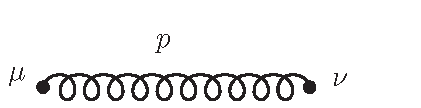
\includegraphics[clip,width=0.2\textwidth]{figures/gp2}
&$\displaystyle ~ \frac{-ig^{\mu\nu}}{p^2}$ \qquad {\footnotesize (Feynman gauge)}\\
    \noalign{\vskip 2mm}
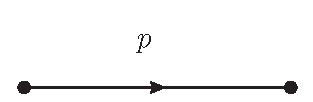
\includegraphics[clip,width=0.15\textwidth]{figures/qp2} &
$\displaystyle  ~ \frac{i(\slashed{p}+m)}{p^2-m^2}$\\
    \noalign{\vskip 4mm}
\raisebox{-.4\height}{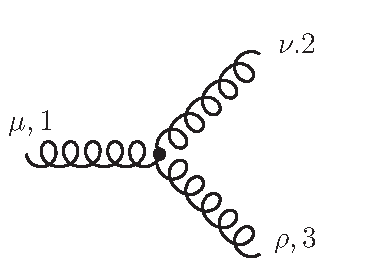
\includegraphics[clip,width=0.2\textwidth]{figures/gggv}}
& $\displaystyle ~ \frac{i}{\sqrt{2}} \left[
        g^{\mu\nu}(p_1-p_2)^\rho+g^{\nu\rho}(p_2-p_3)^\mu+g^{\rho\mu}(p_3-p_1)^\nu\right]$\\
\raisebox{-.4\height}{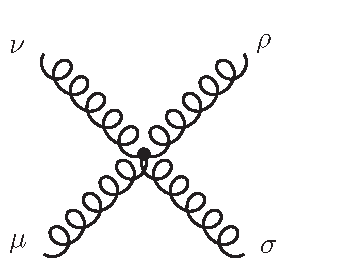
\includegraphics[clip,width=0.2\textwidth]{figures/gggg}}
&  $\displaystyle~ i \left[ g^{\mu\rho}g^{\nu
        \sigma}-\frac{1}{2}(g^{\mu\nu}g^{\rho\sigma}+g^{\mu\sigma}g^{\nu\rho})\right]$ 
\end{tabularx}\\
    \noalign{\vskip 2mm}
\begin{tabularx}{\textwidth}{lp{4.5cm}ll}
\raisebox{-.4\height}{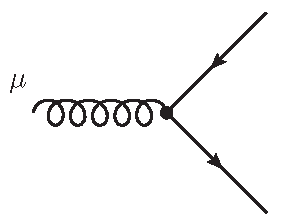
\includegraphics[clip,width=0.15\textwidth]{figures/qqg}}
&
$\displaystyle~ \frac{i}{\sqrt{2}} g_{s} \gamma^{\mu}$&
\raisebox{-.4\height}{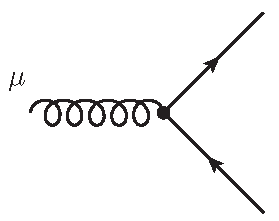
\includegraphics[clip,width=0.15\textwidth]{figures/qqg2}}
&
$ \displaystyle~  -\frac{i}{\sqrt{2}} g_{s} \gamma^{\mu}$\\[1ex]
    \hline
\end{tabularx}
\end{tabular}
\end{table}





\chapter{The van Neerven-Vermaseren Basis}
\label{sec:vNV_basis}

The van Neerven-Vermaseren basis \cite{Neerven1984a,Ellis:2007br}
takes a list of $n<D$ vectors $\{p_1,\ldots{}p_n\}$ as an input, 
and decomposes the full vector space in $D$ dimensions $\mathsf{S}_{[D]}$ into
a direct sum,
\begin{subequations}
  \begin{gather}
    \mathsf{S}_{[D]} = \spn{v_1,\ldots{},v_n} \oplus \spn{\tau_1,\ldots{},\tau_{D-n}},
    \intertext{with $\spn{p_1,\ldots{},p_n} = \spn{v_1,\ldots{},v_n}$, and dual vectors $v_i = \qty(G^{-1})_{ij}\,p_j$, such that}
    \sp(\tau_i,p_j) = \sp(\tau_i,v_j) = 0, \\
    \sp(v_i,p_j) = \delta_{ij}, \qquad \sp(\tau_i,\tau_j) = \delta_{ij} (\tau_{j})^2,
  \end{gather}
\end{subequations}
where $G^{-1}$ is the inverse of the Gram matrix $G_{ij}=\sp(p_i,p_j)$.
The basis vectors of the transverse space $\tau_i$ can be obtained by projecting any $(D-n)$ linear independent seed vectors
into the transverse space with
\begin{align}\label{eq:metricpron}
  g_\tau^{\mu\nu} =  g^{\mu\nu} - \sum_{i=1}^{n}p_i^\mu v_i^\nu,
\end{align}
and orthogonalizing them via the Gram-Schmidt process.

The algorithm works for any dimension $D$ and metric signature.%
\footnote{There are some subtleties connected to non-positive-definite metric signatures (see e.g.\ the bubble topology in \cref{sec:ms_examples})}
It also works over arbitrary field as long as we don't require the transverse vectors to be normalized.


\chapter{Spinor-Helicity}
\label{chap:4dspinhel}

The spinor-helicity methods are covered in great details in numerous sources (e.g.\ \cite{Maitre:2007jq,Kuczmarski:2014ara,Weinzierl:2016bus,DittmaierWeyl,Cohen:2010mi}).
Here we provide only a brief summary.

Helicity of a particle is the projection of it's spin $\va{S}$ on the direction of it's
three-momentum $\va{p}$, and the states $\psi_{\pm s}$ with helicity $\pm s$ are defined as
\begin{equation} \label{eq:helicity_def}
  \sp(\va{S},\va{p}) \, \psi_{\pm s} = \pm s \abs{\va{p}}\, \psi_{\pm s}.
\end{equation}
The helicity of massless particles is a Lorentz invariant, and for spinor representations helicity and chirality eigenstates
coincide. 
%In fact the helicity eigenstates of massless particles are induced unitary representations
For massive particles helicity eigenstates can be constructed relative to a chosen reference frame.


\subsubsection{Massless Spin $1/2$}

For massless spin $\frac{1}{2}$ particles $\va{S} = \frac{1}{2}\va{\sigma}$, and 
the \cref{eq:helicity_def} is written in a covariant way as
\begin{equation}
  (\sp(p,\bar{\sigma}))^{\dot{A}B} \lambda_B(p) = 0, \qquad (\sp(p,\sigma))_{A\dot{B}} \lambda^{\dot{B}}(p) = 0,
\end{equation}
for positive and negative helicities correspondingly.
Here 
\begin{equation}
  \sigma_{A \dot{B}}^{\mu} \coloneqq  \left( 1 , - \vec{\sigma} \right) \qand \bar{\sigma}^{\mu \dot{A} B} \coloneqq  \left( 1 ,  \vec{\sigma} \right),
  \qquad \vec{\sigma}\coloneqq (\sigma_x,\sigma_y,\sigma_z),
\end{equation} 
with the standard Pauli matrices
\begin{eqnarray}
  \sigma_x = \left(\begin{array}{cc}
    0 & 1\\
    1 & 0 \\
  \end{array} \right),
  &
  \sigma_y = \left(\begin{array}{cc}
    0 & -i\\
    i & 0 \\
  \end{array} \right),
  &
  \sigma_z = \left(\begin{array}{cc}
    1 & 0\\
    0 & -1 \\
  \end{array} \right),
\end{eqnarray}
and we introduced dotted and undotted spinor indices corresponding to the two non-equivalent representation of $SL(2,\mathbb{C})$.
The indices can raised and lowered with the 2-dimensional Levi-Civita symbol as
\begin{equation}
    \label{raising_and_lowering_spinor_indices}
  \begin{gathered}
    p^A = \varepsilon^{AB} p_B, \qquad
    p^{\dot{A}} = \varepsilon^{\dot{A}\dot{B}} p_{\dot{B}}, \\
    p_{\dot{B}} = p^{\dot{A}} \varepsilon_{\dot{A}\dot{B}},  \qquad
    p_B = p^A \varepsilon_{AB},
  \end{gathered}
\end{equation}
which satisfies the properties
\begin{equation}
  \begin{gathered}
    \varepsilon_{BA} = - \varepsilon_{AB},  \quad   \varepsilon^{AB} = \varepsilon^{\dot{A}\dot{B}} = \varepsilon_{AB} = \varepsilon_{\dot{A}\dot{B}}, \\
    \eps^{A C} \eps_{B C} = \delta^{A}_{\;B}, \quad \eps^{\dot{A} \dot{C}} \eps_{\dot{B} \dot{C}} = \delta^{\dot{A}}_{\;\dot{B}}.
  \end{gathered}
\end{equation}
We will use a convenient notation of angle and square brackets,
\begin{equation}
  \begin{aligned}
    \ket{p} &\coloneqq \lambda_A(p) = u_+(p) = v_-(p) , \qquad &\bra{p} \coloneqq \lambda^A(p) = \bar{u}_-(p) = \bar{v}_+(p),  \\
    \sket{p} &\coloneqq \lambda^{\dot{A}}(p) = u_-(p) = v_+(p), \qquad &\sbra{p} \coloneqq \lambda_{\dot{A}}(p)= \bar{u}_+(p) = \bar{v}_-(p),
  \end{aligned}
\end{equation}
to write compactly the spinor products,
\begin{subequations}
  \begin{equation}
    \spaa(p,q) \coloneqq \lambda^A(p) \lambda_A(q), \qquad \spbb(p,q) \coloneqq \lambda_{\dot{A}}(p) \lambda^{\dot{A}}(q),
  \end{equation}
  and spinor chains such as
  \begin{equation} \label{eq:vectors_from_spinors}
    \sbraket(p,\gamma^\mu,q) = \brasket(q,\gamma^\mu,p)  \coloneqq \lambda_{\dot{A}}(p) \bar\sigma^{\mu\dot{A}B} \lambda_B(q).
  \end{equation}
\end{subequations}

Explicitly, the components of spinors are given as
\begin{equation}
  \lambda_A = t \frac{1}{\sqrt{p_+}}\begin{pmatrix} p_+ \\ p^\perp_+ \end{pmatrix}, \quad \lambda_{\dot{A}} = \frac{1}{t}\frac{1}{\sqrt{p_+}}\begin{pmatrix} p_+ \\ p^\perp_- \end{pmatrix},
\end{equation}
where 
\begin{equation}
  p_{\pm} \coloneqq p_0 \pm p_3, \qquad p^\perp_{\pm} \coloneqq p_1 \pm i\,p_2,
\end{equation}
and $t$ is an arbitrary little-group scaling factor, and for real $p$, $\abs{t}=1$.
As long as we are considering Lorentz-invariant quantities (e.g.\ helicity amplitudes normalized by their spinor weight),
we can get the same results by operating with \emph{denormalized} spinors instead
\begin{equation}
  \tilde\lambda_A \coloneqq  \begin{pmatrix} p_+ \\ p^\perp_+ \end{pmatrix}, \quad \tilde\lambda_{\dot{A}} \coloneqq  \frac{1}{p_+}\begin{pmatrix} p_+ \\ p^\perp_- \end{pmatrix}.
\end{equation}
This can be exploited to not evaluate the squre root in computations over finite fields.




\subsubsection{Massless Spin 1}

It is easy to see, that the spinor chains of the form of \cref{eq:vectors_from_spinors} are light-like Lorentz vectors.
The helicity eigenstates of vector particles can be constructed as
\begin{equation}
  \varepsilon_+^\mu(p,\eta) = -\frac{\sbraket(p,\gamma^\mu,\eta)}{\sqrt{2} \spaa(p,\eta)}, \qquad \varepsilon_-^\mu(p,\eta) = \frac{\brasket(p,\gamma^\mu,\eta)}{\sqrt{2} \spbb(p,\eta)},
\end{equation}
where $\eta$ is some arbitrary reference vector. Indeed
the relations 
\begin{equation}
  \qty(\varepsilon_{\pm})^2 =0, \qquad
  \varepsilon^{\mu}_{\pm}(p,\eta) p_\mu = 0,
  \;\;\;\;
  \varepsilon^{\mu}_{\pm}(p,\eta) \eta_\mu = 0,
\end{equation}
are satisfied by construction, and the polarization sum is
\begin{equation}
  \varepsilon^{\mu}_{+}(p,\eta)\varepsilon^{\nu}_{-}(p,\eta) + \varepsilon^{\mu}_{-}(p,\eta)\varepsilon^{\nu}_{+}(p,\eta) = -g^{\mu\nu} + \frac{\ell^\mu \eta^\nu + \ell^\nu \eta^\mu}{\sp(\ell,\eta)}.
\end{equation}
The little group scaling is
\begin{equation}
  \varepsilon_{\pm} \longrightarrow t^{(\mp 2)} \varepsilon_{\pm},
\end{equation}
as it should be.


\subsubsection{Massive Spin 1/2}

Given any time-like momentum $p$ with $p^2 = m^2$, and a light-like reference vector $q$, we can perform a light-cone decomposition of $p$ 
into a sum of two light-like vectors,
\begin{equation}
  p = p^q + \frac{m^2}{2 \sp(p,q)} q, \qquad (p^q)^2 = q^2 = 0, \qquad \sp(p,q) = \sp(p^q,q).
\end{equation}
The spinors associated to $p_q$ are found as
\begin{equation}
  \ket{p^q} = t_q \frac{1}{\sqrt{2\sp(p,q)}} \; \slashed{p} \ket{q},  \qquad \sket{p^q} = \frac{1}{t_q} \frac{1}{\sqrt{2\sp(p,q)}} \; \slashed{p} \sket{q},
\end{equation}
with the corresponding little-group scaling $t_q$.

Dirac spinors with momentum $p$ (in the Weyl representation) are then given by
\begin{equation} \label{eq:massive-spinors}
  \begin{aligned}
    \bar{u}_{+}(p) &= \sbra{p^q} + \frac{m}{\spaa(q,p^q)} \bra{q},  &\qquad  v_{+}(p) &= \sket{p^q} - \frac{m}{\spaa(p^q,q)} \ket{q}, \\
    \bar{u}_{-}(p) &= \bra{p^q} + \frac{m}{\spbb(q,p^q)} \sbra{q},   & v_{-}(p) &= \ket{p^q} - \frac{m}{\spbb(p^q,q)} \sket{q}.
  \end{aligned}
\end{equation}
In the limit $m\to 0$, by construction $p \to p^q$, and the above spinors become independent of the reference vector $q$ and reduce to the corresponding massless spinors.
Evidently, the helicity amplitudes evaluated with the states from \cref{eq:massive-spinors} scale under the little group as their reference spinors.



\chapter{Clifford Algebras in $D_s$ Dimensions}
\label{sec:clifford_algebra_ds}

\section{Representations}
The defining property of the Clifford algebra is
\begin{equation} \label{eqn:defClifford}
\acomm{\gamma_{[D_s]}^\mu}{\gamma_{[D_s]}^\nu} = 2 g_{[D_s]}^{\mu\nu}\mathbb{1}_{[D_s]}^{\vphantom{\mu\nu}},
\end{equation}
where $\mathbb{1}_{[D_s]}$ is the identity of the Clifford algebra.
The representations are constructed via recursive application of tensor products (see e.g.\ refs.~\cite{Collins:1984xc,Kreuzer:susylectures}):
\begin{align}\label{eq:gammait}
  \gamma^\mu_{[Ds]}  = 
  \begin{dcases}
    \mathbb{1}_{[2]} \otimes \gamma^\mu_{[D_s-2]}, & \mu =0\leq D_s-3,\\
    (\sigma_2\,\sigma_3) \otimes \gamma^\star_{[D_s-2]}, & \mu = D_s-2,\\
    (\sigma_3\,\sigma_1) \otimes \gamma^\star_{[D_s-2]}, & \mu = D_s-1,\\
  \end{dcases}
\end{align}
where $\{\sigma_1,\sigma_2,\sigma_3\}$ are Pauli matrices, and
\begin{equation}
  \begin{gathered}
    \gamma^\star_{[D_s]} \coloneqq i^{\frac{D_s}{2}-1} \gamma^0_{[D_s]}\cdots{}\gamma^{D_s -1 }_{[D_s]} ~\equiv~ \sigma_3 \otimes \gamma^\star_{[D_s-2]}, \\
    \acomm{\gamma^\star_{[D_s]}}{\gamma^\mu_{[D_s]}}=0, \qquad \gamma^\star_{[D_s]} \gamma^\star_{[D_s]} = \mathbb{1}_{[D_s]}.
  \end{gathered}
\end{equation}
We can thus write the Clifford algebra in $D_s$ dimensions in a factorized way,
\begin{equation}\label{eqn:cliffordrecursion}
  \qty(\gamma_{[D_s]}^\mu)_{a\kappa}^{\,b\lambda}  =
  \begin{dcases}
    \qty(\gamma_{[4]}^\mu)_a^{\;b} \, \delta_\kappa^\lambda\,, &  0\le\mu \le 3 \,,\\
    \qty(\gamma^{\star}_{[4]})_a^{\;b} \qty(\gamma_{[D_s-4]}^{(\mu-4)})_\kappa^{\;\lambda}\,, & \mu>3 \,,
  \end{dcases}
\end{equation}
where the indices $a,b$ denote the spinor indices in $\mathsf{S}_{[4]}$ and $\kappa,\lambda$ the ones in $\mathsf{S}_{[D_s - 4]}$.
Note that $\gamma^\mu_{[D_s-4]}$ represent a $(D_s-4)$-dimensional Clifford algebra.

%The spinor states for a particle with momentum $p$ satisfy the Dirac equation
%\begin{equation}
  %\qty(\slashed{p}_{[D_s]} \pm m \cdot \mathbb{1}_{[D_s]}) \psi  = 0,
%\end{equation}
\section{Basis and Certain Traces}
\label{sec:identities}

We derive the coefficients $c_n(D_s-4)$ from \cref{eq:dsm_4_projectors} for
the case of two external non-identical fermion lines.
For convenience, in this \namecref{sec:identities} we denote
\begin{equation}
  d \coloneqq D_s-4, \qquad  d_t \coloneqq \Tr(\mathbb{1}_{[d]})=2^{d/2}.
\end{equation}
The factor $d_t$ is always factorized from the amplitude, so it is usually set to $1$ in dimensional regularization \cite{Collins:1984xc}.
Here we will keep it for clarity, since we are considering a finite-dimensional Clifford algebra.
We choose the basis of the Clifford algebra as
\begin{align}\label{eq:basisGammaChainII}
\gamma_{[d]}^{\mu_1 \ldots \mu_n} = \frac{1}{n!} \sum_{ \sigma\in
S_n} \sgn(\sigma) \gamma_{[d]}^{\mu_{\sigma(1)}} \ldots
\gamma_{[d]}^{\mu_{\sigma_n}}\,,
\end{align}
From the properties of $\gamma$-matrices we have
\begin{eqnarray}
  (\gamma_{[d]}^{\mu_1 \ldots \mu_n} )^\dagger =\,
  \gamma_{[d]\mu_n \ldots \mu_1}^{\phantom{\mu}} \,,
\end{eqnarray}
and the following result for the traces can be derived (see e.g.\ \cite{Veltman:1988au}):
\begin{eqnarray}
  \label{eq:traceChain}
  \Tr(\gamma_{[d]}^{\mu_1 \ldots \mu_n} \gamma^{
    \phantom{\mu}}_{[d]\,\nu_m \ldots \nu_1})= 
    \left\{ \begin{array}{cc} d_t 
      \sum_{ \sigma\in  S_n} \sgn(\sigma)
      \delta^{\mu_{\sigma(1)}}_{\nu_1}\cdots\delta^{\mu_{\sigma(n)}}_
      {\nu_n} &\qquad m=n   \\
      0 &\qquad m\neq n\end{array}  
    \right. 
    \,,
  \end{eqnarray}
%
where the summation runs over all permutations $S_n$ of $n$ elements.
We will also need the following identity for contracted Lorentz indices:
\begin{eqnarray}
  \label{eqn:simpletrace}
  \sum_{\mu_1,\ldots,\mu_n} 
  \sum_{ \sigma\in  S_n} \sgn(\sigma)
  \delta^{\mu_{\sigma(1)}}_{\mu_1}\ldots
  \delta^{\mu_{\sigma(n)}}_{\mu_n}
  = \frac{d!}{(d-n)! }\,.
\end{eqnarray}
The sum counts the number of antisymmetric tensors of
rank $n$ in $d$ dimensions, which is the number of ways to 
choose an ordered subset of $n$ elements from a fixed set of $d$
elements.
%
We now compute the diagonal projections of $v_n$ tensors from \cref{eqn:4qtensors}
which yield the normalisation factors $c_n$ in \cref{eq:dsm_4_projectors}:
\begin{align}
  \begin{split}
    \label{eq:cnCalc}
    c_n=\mathcal{P}_n [v_n] =&\,
%
    \Tr(\gamma_{[d]\,\mu_n \ldots \mu_1} \gamma_{[d]}^
    {\nu_1 \ldots \nu_n}) \,
%
    \Tr(\gamma_{[d]}^{\mu_n \ldots \mu_1} \gamma_{
    [d]\,\nu_1 \ldots \nu_n}) \\
    =&\,
    d_t^2 \sum_{\sigma\in  S_n} 
    \sum_{\mu_1,\ldots,\mu_n}
    \sum_{\tilde \sigma\in S_n}
    \sum_{\nu_1,\ldots,\nu_n}
%
    \sgn(\sigma)
    \sgn(\tilde\sigma)
    \delta^{\mu_{\sigma(n)}}_{\nu_1}\cdots\delta^{\mu_{\sigma(1)}}_{\nu_n}
    \delta_{\mu_{\tilde\sigma(n)}}^{\nu_1}\cdots
    \delta_{\mu_{\tilde\sigma(1)}}^{\nu_n}
    \\
%
    =&\,d_t^2 \sum_{\sigma\in  S_n} 
    \sgn(\sigma)
    \left(
    \sum_{\mu_1,\ldots,\mu_n}\sum_{\tilde \sigma\in S_n}
%
    \sgn(\tilde\sigma)
    \delta^{\mu_{\sigma(n)}}_{\mu_{\tilde\sigma(n)}}
    \cdots
    \delta^{\mu_{\sigma(1)}}_{\mu_{\tilde\sigma(1)}}
    \right)
    \\
%
    =&\, d_t^2 \sum_{\sigma\in  S_n} 
    \sgn(\sigma)^2 \frac{d!}{(d-n)!}\\
    =&\, d_t^2 \frac{d!\,n!}{(d-n)!}\,.
  \end{split}
\end{align}
As expected, for each $n$ the result has zeros in the dimensions
$d$, for which there are insufficient distinct labels 
$\mu_i$ and $\nu_i$ available to form antisymmetric index 
configurations of $n$ indices.



\chapter{Parametrization of Integrands of Amplitudes with External Fermions}
\label{sec:ParamIntegrands}

In this \namecref{sec:ParamIntegrands} we show
explicitly how the Lorentz-invariance of the coefficients $A_n^{(k)}$ of the
tensor tensor decomposition in \cref{eq:tensorDecomposition} guarantees that
no explicit loop-momenta components will appear in the parametrization of their integrands.

%Since our representation of fermion amplitudes is manifestly
%Lorentz invariant in $(D_s-4)$ dimensions prior to loop
%integration, the integrands of fermion amplitudes can be
%decomposed in terms of the same set of master integrands and
%surface terms as those used for amplitudes with gluons only \cite{Abreu:2017xsl,Abreu:2017hqn}.
%We demostrate this below.

The integrand of $\mathcal{A}^{(2)}_{\{k\}}(\ell_l)$ of a two-loop amplitude with an arbitrary
number of quark lines can be schematically written in terms of tensors $f^{\rho_1 \ldots \rho_n, \sigma_1\ldots \sigma_m}_{\{k\}}$ as
\begin{equation} 
  \mathcal{A}_{\{k\}}(\ell_l) = \sum_{n,m} f^{\rho_1 \ldots \rho_n, \sigma_1 \ldots \sigma_m}_{\{k\}}
  \left(\prod_{i=1}^n \vec{\mu}_{1 \, \rho_i}\right)
  \left(\prod_{j=1}^m \vec{\mu}_{2 \, \sigma_i}\right),
\end{equation}
where the indices $\{k\}$ denote all spinor indices in  $\mathsf{S}_{[D_s-4]}$,
and all contractions with the $(D_s-4)$-dimensional part of the loop momenta made explicit.
Upon the projection onto any coefficient by $v_n^\dagger$ we get the sum of products of the metric tensors in $\mathsf{S}_{[D_s-4]}$
from traces of products of $\gamma_{[D_s-4]}$, so 
\begin{equation}
  v_n^\dagger f^{\rho_1 \ldots \rho_n, \sigma_1 \ldots \sigma_m}_{\{k\}}  = \sum_{s\in S_2} c_s \qty(\prod_{\{\alpha_1,\alpha_2\}\in s} g^{\alpha_1,\alpha_2}_{[D_s-4]}),
\end{equation}
where the sum is over all possible ways to pair the indices $\{ \rho_1 \ldots \rho_n,\,\sigma_1 \ldots \sigma_m \}$.
Inserting this into the previous equation we see that only on the invariants $\mu_{ij}$ appear in the integrand of $A_n^{(k)}$.



\chapter{Momentum Twistor Variables}
\label{sec:twistors}

Here we explicitly specify the twistor parametrization~\cite{Hodges:2009hk}, which
we employed to rationalize the external on-shell momenta $\{p_i\}_{i=1,5}$ with
$p_i^2=0$. This parametrization yields a momentum point with the
kinematic invariants $(s_{12}, s_{23}, s_{34}, s_{45}, s_{51})$ from the
input variables $\{ s_{23}, s_{45}, s_{51}, x \}$ and $s_{12}=1$ 
as given in the main text in eq.~\eqref{eq:s34Definition}.

Using the notation from \cref{chap:4dspinhel}, the momenta $p_i$ are written in terms of spinors as
\begin{equation}
  p^\mu_i = \frac{1}{2}\sbraket(i,\gamma^\mu,i) = \frac{1}{2}\brasket(i,\gamma^\mu,i)
\end{equation}

We introduce an auxiliary spinors $\sket{\mu_i}$,
such that the spinors $\ket{i}$, $\sket{\mu_i}$ are parametrized by the matrix,
\begin{equation}
  \begin{pmatrix}
    \ket{1} &  \ket{2} &   \ket{3} &   \ket{4} &  
    \ket{5} \\   
    \sket{\mu_1} &  
    \sket{\mu_2} &  
    \sket{\mu_3} &  
    \sket{\mu_4} &  
    \sket{\mu_5} 
  \end{pmatrix}
  =
  \begin{pmatrix}
    1 & 0 & 1 & 1 \!+\! \frac{1}{x}  &  1 \!+\! \frac{1}{x} \!+\! \frac{x-s_{23}+s_{45}}{x s_{51}}\\
    0 & 1 & 1 & 1                    &  1\\
    0 & 0 & 0 & \frac{s_{23}}{x}     &  1\\
    0 & 0 & 1 & 1                    & 1 \!-\! \frac{s_{45}}{s_{23}}
  \end{pmatrix}
  \label{eq:TwistorParametrization}
\end{equation}
%
The spinors $\sbra{i}$ are then obtained as
\begin{equation}
\sbra{i} = \frac{\langle i, i+1 \rangle \sbra{\mu_{i-1}} + \langle i+1, i-1\rangle \sbra{\mu_{i}} + \langle i-1, i \rangle\sbra{\mu_{i+1}}}{\langle i, i+1\rangle \langle i-1, i\rangle}\, .
\end{equation}





\chapter{Numerical Algorithms}

Here we provide a brief summary of the numerical algorithms, which we employed in out computations.


\section{Finite Fields}
\label{sec:ff_fp}

The numerical unitarity method, which we presented in \cref{chap:numunitarity}, is suitable 
for evaluations in any number field.\footnote{
  With a caveat discussed in \cref{sec:muij_square_roots}
}
One particularly useful choice is that of finite fields $\mathbb{Z}_p$, with the prime cardinality $p$,
which  can be chosen such that all elements of the field fit into the standard machine integer.
This allows to carry out arithmetics efficiently.

A rational number $x=\frac{n}{d}$ is mapped into $\mathbb{Z}_p$ as
\begin{equation}
  x \to \frac{n\mod{p}}{d\mod{p}},
\end{equation}
and the division in $\mathbb{Z}_p$ is implemented with the extended Euclidean algorithm.

The inverse map exists \cite{Wang:1981:PAU:800206.806398} only if $\abs{n},\abs{d} < \sqrt{\frac{p}{2}}$.
However, with the help of the Chinese Remainder Theorem, the images of $x$ in multiple finite fields $\mathbb{Z}_{p_i}$
can be combined to get an image in $\mathbb{Z}_{\prod_i p_i}$.
This procedure is called \emph{rational reconstruction}. 
We refer to further details elsewhere \cite{Klappert:2019emp,Peraro:2016wsq}

\begin{figure}[ht]
  \begin{center}
    \begin{tikzpicture}[auto, node distance = 3cm,shorten >= 2pt]
      \node [rectangle, draw, text centered] (x) {$\mathbf{x}$};

      \node [above right = 0.3cm and 0.7cm of x] (xmod1) {$\mathbf{x}\mod p_1$};
      \node [right  of=xmod1] (cmod1) {$c\mod p_1$};

      \node [below right = 0.3cm and 0.7cm of x] (xmodn) {$\mathbf{x}\mod p_n$};
      \node [right  of=xmodn] (cmodn) {$c\mod p_n$};


      \node [below = 0cm of xmod1] () {$\vdots$};
      \node [below = 0cm of cmod1] () {$\vdots$};
      \node [below right = 0cm and 0.1cm of xmod1] () {$\vdots$};

      \node [ellipse, draw, text centered, right =6cm of x, node distance = 3cm, text width = 1.5cm, inner sep = 1pt] (crt) {\baselineskip=-10pt \tiny Chinese Remainder Theorem \par};
      \node [right = 0.5cm of crt] (cmodP) {\minibox{ $c\mod P$  \\ \footnotesize $\left(P\coloneqq\prod_i p_i\right)$} };

      \node [rectangle, draw, text centered, right of=cmodP, node distance = 3cm] (c) {$c$};


      \path [line,->] (x) -- (xmod1.west);
      \path [line,->] (x) -- (xmodn.west);

      \path [line,->] (xmod1.east) -- node [above]{$f$} (cmod1.west);
      \path [line,->] (xmodn.east) -- node [above]{$f$} (cmodn.west);

      \path [line,->] (cmod1.east) -- (crt);
      \path [line,->] (cmodn.east) -- (crt);

      \path [line,->] (crt) -- (cmodP);

      \path [line,->] (cmodP) -- node [above]{\small $n,d < \sqrt{\frac{P}{2}}$} (c);
    \end{tikzpicture}
  \end{center}
  \caption{The diagram, representing the evaluation of any rational function from a sample of finite fields.}
  \label{fig:RatReconstr}
\end{figure}


Any rational function $f: \mathbb{Q} \longrightarrow \mathbb{Q}$ can be reinterpreted
to be a function $f: \mathbb{Z}_p \longrightarrow \mathbb{Z}_p$.
We can then use the rational reconstruction algorithm to obtain the value $c = f(\vb*{x}) = \frac{d}{n}$
from its finite-field images. This is illustrated in \cref{fig:RatReconstr}.
A finite-field based calculation allows to compute exact values
for the coefficients $c_{\Gamma,i}$ in \eqref{eq:cut_equations}.


\section{On-Shell Loop Momenta and Finite Fields}
\label{sec:muij_square_roots}

In \cref{sec:osm} we discussed the algorithm for
finding on-shell loop momenta for generic topologies.
Our parametrization trivializes on-shell conditions for the components
of loop momenta $\ell^{\mu}_{l[4]}$, and provides
the \emph{quadratic} constraints for the components $\vec{\mu}_l \coloneqq \ell^{\mu}_{l[D-4]}  $,
\begin{equation} \label{eq:vecmu_conditions}
  \va{\mu}_i \cdot \va{\mu}_j  \equiv  \mu_{ij} (\vb*{\rho},\vb*{\alpha}) = \ell_i\cdot \ell_j - \ell_{i[4]}\cdot \ell_{j[4]},
\end{equation}
In general, quadratic equations do not have solutions in an arbitrary field $\mathbb{F}$.
To address this issue, we will consider an algebraic extension of the field $\mathbb{F}$.
We choose an orthonormal
basis $\{\vec{n}_i\}$ in $\mathsf{S}_{[D-4]}$ such that
\begin{equation}
\vec{\mu}_1 = r_1 \vec{n}_1, \quad  \vec{\mu}_2 = \frac{\mu_{12}}{\mu_{11}} r_1 \vec{n}_1 + r_2 \vec{n}_2
  \quad \mathrm{with} \quad r_1 = \sqrt{\mu_{11}}, \quad r_2 = 
  \sqrt{\mu_{22} - \frac{\mu_{12}^2}{\mu_{11}}},
\end{equation}
Then conditions \cref{eq:vecmu_conditions} are satisfied by construction.
The components of off-shell currents will take the generic form
\begin{equation}
  \label{eq:ExtendedAlgebra}
  a_{00} + a_{10} r_1 + a_{01} r_2 + a_{11} r_1 r_2, 
\end{equation}
which is not $\mathbb{F}$-valued.
Then, in order to nevertheless be able to
work in the field $\mathbb{F}$, we consider 
the algebra $\mathbb{V}$ over the field $\mathbb{F}$, with 
the vector space $\mathbb{V}$ spanned by the basis 
$\{r_0=1,r_1,r_2,r_1r_2\}$ and equipped with the standard
addition and multiplication.
All components of the off-shell currents are elements 
of the algebra $\mathbb{V}$, and can thus be written as linear combinations
of $r_i$ with $\mathbb{F}$-valued coefficients. More
concretely, this means we only need to determine the $a_{ij}$ 
in \cref{eq:ExtendedAlgebra} which are $\mathbb{F}$-valued
by construction.

An important observation is that, although the coefficients 
$a_{10}$, $a_{01}$ and $a_{11}$ in 
\cref{eq:ExtendedAlgebra} are non-zero in
intermediate stages of the calculations of cuts, they vanish
for the integrands of helicity amplitudes as defined in 
\cref{eq:tensorDecomposition}. This cancellation of the
$r_i$ terms holds in the HV scheme and
is due to the projection onto the invariant tensors 
$v_n$ of \cref{eq:tensorDecomposition}, 
which yields polynomials in the Lorentz invariants 
$\mu_{ij}$ at the integrand level.


\subsubsection{The Case of Only Vector Particles}
%
It was shown in \cite{Abreu:2017hqn}, that,
if only vector particles are encountered in the computation of cuts,
the off-shell recursion can be modified to work directly with scalar products $\mu_{ij}$.
Hence, the square roots $r_i$ do not appear explicitly.
More precisely, this corresponds to choosing to work with orthogonal, but not normalized basis $\{\tilde{\vec{n}}_j\}$ in
$\mathsf{S}_{[D-4]}$,
\begin{equation}
  \tilde{\vec{n}}_1 = r_1 \begin{pmatrix} 1 \\ 0\end{pmatrix}, \qquad \tilde{\vec{n}}_2 = r_2 \begin{pmatrix} 0 \\ 1 \end{pmatrix}
\end{equation}


\subsubsection{Special Metric Signature}
In the presence of fermions, the situation becomes more 
complicated, due to the extension of the Clifford algebra beyond 
four dimensions. More specifically, terms such as $\slashed{\ell}_{[D_s]}$
exhibit the $(D-4)$-dimensional components of the loop momenta.
Thus, we need to use the algebraic extension in \cref{eq:ExtendedAlgebra}.
We can however reduce the number of square roots by a trivial reparametrization, taking advantage of a particular choice
of metric signature.

Any Lorentz-invariant quantity depends on the space-time metric tensor only through contractions with momenta and states of external particles.
Thus  without loss of generality we can choose to use an alternating metric signature $(+,-,+,-,\ldots)$,
and modify external momenta such that all Lorentz invariants remain unchanged.
We then can parametrize the two-dimensional loop-momentum components
$\vec{\mu}_1$ and $\vec{\mu}_2$ as follows:
\begin{equation}
  \vec{\mu}_1(t)  = \frac{1}{2}\begin{pmatrix}
    t+\dfrac{\mu_{11}}{t} \\
    t-\dfrac{\mu_{11}}{t} \\
  \end{pmatrix}, \quad
  \vec{\mu}_2(t)  = \frac{\mu_{12}}{\mu_{11}}\vec{\mu}_1(t) - \frac{r}{\mu_{11}}~\frac{1}{2}\begin{pmatrix}
    t-\dfrac{\mu_{11}}{t} \\
    t+\dfrac{\mu_{11}}{t} \\
  \end{pmatrix},
  \label{eq:muparam}
\end{equation}
where $t$ is a free dimensionful parameter that leaves the scalar products
$r = \sqrt{\mu_{12}^2-\mu_{11} \mu_{22}}$ and 
$\mu_{ij} = \mu_i^1 \mu_j^1 - \mu_i^2 \mu_j^2$ invariant. %


\section{Exact Interpolation of Functions over Finite Fields}
\label{sec:func_reconstruction}
{
\newcommand{\nn}{\\}
We give a brief overview of the function interpolation (or analytic reconstruction) techniques, that we used to obtain the analytic expressions in \cref{sec:AnalyticForm} from exact numerical evaluations over finite fields.
We stress, that the analytic reconstruction reproduces the sampled function exactly.
This means, that the subsequent numerical evaluations will always agree exactly with the reconstructed function.
We refer for details to \cite{Klappert:2019emp,Peraro:2016wsq,Peraro:2019svx}.

\subsection{Univariate Polynomials}
\label{sec:newton}

The analytic reconstruction of a dense univariate polynomial $f(x) \in \mathbb{Z}_p[x]$ of unknown degree can be done with the Newton interpolating polynomials.
The polynomial is represented in the form
\begin{align*}
  f(x)    &= \sum_{r=0}^Ra_r\prod_{i=0}^{r-1}(x-y_i) \\
  &= a_0 + (x-y_0) 
  \Bigg( 
  a_1 + (x-y_1) 
  \Big( 
  a_2 + (x-y_2) (\dots + (x-y_{R-1})a_R)
  \Big)
  \Bigg)
\end{align*}
where $y_{j} \in \mathbb{Z}_p$ are the sample points.
The coefficients $a_k$ are then determined recursively as 
\begin{align*} %\label{eq:newtonsystem}
  a_0 ={}& f(y_0) \nn
  a_1 = {} & \frac{f(y_1)-a_0}{y_1-y_0} \nn
  & \vdots  \\
  a_i = {} & \Bigg(\Big(\big(f(y_i)-a_0\big) \frac{1}{y_i-y_0}-a_1\Big) \frac{1}{y_i-y_1}-\cdots - a_{i-1} \Bigg) \frac{1}{y_i-y_{i-1}}.
\end{align*}
Note, that the degree $R$ of the polynomial is uncovered with this procedure.

\subsection{Multivariate Polynomials}
\label{sec:newton_rec}

The analytic reconstruction of a dense multivariate polynomial $f(\vb*{x})$ of unknown degree can be done with the recursive application of the univariate Newton formula.
In the first step we put all, but the first variable to some values and perform a univariate reconstruction in $x_1$,
\begin{equation} %\label{eq:mnewtonrep}
  f(\vb*{x}) ={} \sum_{i=0}^R a_i(x_2,\ldots,x_n) \prod_{j=0}^{i-1} (x_1-y_j).
\end{equation}
We then apply the same argument to $a_i(x_2,\ldots,x_n)$, ans so on.

\subsection{Univariate Rational Function}
\label{sec:thiele}

Analogous to the case of univariate polynomials,
the analytic reconstruction of a dense univariate rational function 
\begin{equation} \label{eq:defuratfun}
  f(x) = \frac{\sum_{i=0}^{R_n} n_i\, x^i}{\sum_{i=0}^{R_d} d_{i}\, x^{i}},
\end{equation}
of unknown degree can be done with the Thiele's formula  \cite{Abramowitz1964}.
The function is represented in the form
\begin{align} \label{eq:thielerep}
  f(x) = {} & a_0 + \dfrac{x-y_0}{a_1 + \dfrac{x-y_1}{a_2 + \dfrac{x-y_3}{\cdots + \dfrac{x-y_{N-1}}{a_N}}}} \nn
       = {} & a_0 + (x-y_0)\left(a_1 + (x-y_1)\left( a_2 + (x-y_2) \left(\cdots+ \frac{x-y_{N-1}}{a_N}\right)^{-1} \right)^{-1} \right)^{-1},
\end{align}
with $N = 2\max(R_n,R_d)$.
This is due to the fact, that the numerator's and denominator's degrees differ at most by $1$ in the Thiele's formula.
The coefficients $a_i$ are obtained as
\begin{align*} %\label{eq:thielesolve}
  a_0 ={}& f(y_0) \nn
  a_1 = {} & \frac{y_1-y_0}{f(y_1)-a_0} \nn
  & \vdots{} \\
  a_i = {} & \left(\left(\left(f(y_i)-a_0\right)^{-1}(y_i-y_0)-a_1\right)^{-1} (y_i-y_1)-\cdots -a_{i-1}\right)^{-1} (y_i-y_{i-1}).
\end{align*}
As for Newton polynomials, the degrees $R_n$ and $R_d$ of the rational function are uncovered with this procedure.

%We  observethat  Thiele’s  formula  withN+ 1  terms  represents  a  rational
%function  with  degreeRandR′for the numerator the denominator respectively,
%whereR=R′=N/2 ifNis even, andR=R′+ 1 = (N+ 1)/2 ifNis odd.  In other words,
%either the degree of the numerator andthe denominator of the reconstructed
%function are equal, or they differ by one unity at most.This implies that the
%highest degree coefficientsnrordr′, obtained by converting the resultinto its
%canonical form, might be vanishing, in which case they are discarded. 

}
